% Diese Vorlage wurde von Simon Berwert erstellt. Weitere Erkl�rungen findest du auf folgender Seite: http://www.unimac.ch/students/latex.de.html



% A. PR�AMBEL
% ***************************************************************************************************

\documentclass[smallheadings,headsepline, titlepage,12pt,a4paper]{scrartcl}
% Hier gibt man an, welche Art von Dokument man schreiben m�chte.
% Möglichkeiten in {}: scrartcl, scrreprt, scrbook, aber auch: article, report, book
\usepackage[ngerman]{babel} % erm�glicht deutsche Silbentrennung und direkte Eingabe von Umlauten, ...
\usepackage{ucs}
\usepackage[ansinew]{inputenc} % teilt LaTeX die Texcodierung mit. Bei Windowssystemen: ansinew
\usepackage[T1]{fontenc} % erm�glicht die Silbentrennung von Wörtern mit Umlauten
\usepackage{hyperref} % PDF wird mit Lesezeichen (verlinktes Inhaltsverzeichnis) versehen (bei Betrachtung mit Acrobat Reader sichtbar)
\typearea{12} % Breite des bedruckten Bereiches vergr�ssern (funktioniert nur in \documentclass mit: scrreprt, scrartcl, scrbook)
\pagestyle{headings} % schaltet Kopfzeilen ein
\clubpenalty = 10000 % schliesst Schusterjungen aus
\widowpenalty = 10000 % schliesst Hurenkinder aus
%\usepackage{geometry}
%\geometry{lmargin=2cm,rmargin=2cm,tmargin=1cm,bmar gin=1cm,headheight=0ex}
\usepackage{longtable} % erm�glicht die Verwendung von langen Tabellen
\usepackage{graphicx} % erm�glicht die Verwendung von Graphiken.
\usepackage{times}
\usepackage{listings}
\lstloadlanguages{Java}
\lstdefinestyle{java}{
        language=Java,
        escapeinside={(*@}{@*)},
        frameround=tttt,
        frame=tRBl,
        numbers=left,
        stepnumber=1,
        numberstyle=\tiny,
        basicstyle=\small\sffamily,
        commentstyle=\slshape,
        columns=fullflexible,
        keepspaces=true,
        fontadjust=true,
        morecomment=[l]{--},
%        literate=
%                {>}{{$>$}}1
%                {<}{{$<$}}1
%                {\\}{{$\lambda$}}1
%                {->}{{$\rightarrow$}}2
}
\lstset{numbers=none,
        numberstyle=\tiny,
        numbersep=5pt,
        basicstyle=\small,        
        xleftmargin=0.4cm,
        breaklines=true,
        captionpos=b}
\usepackage{color}
\newcommand{\thesame}{\color{red}\ttfamily}%
\newcommand{\red}{\color{red}\ttfamily}%
\newcommand{\blue}{\color{blue}\ttfamily}%
\begin{document}

% B. TITELSEITE UND INHALTSVERZEICHNIS
% ***************************************************************************************************

\titlehead{Universit�t Koblenz-Landau\\
Institut f�r Softwaretechnik\\
Universit�tsstr. 1\\
56072 Koblenz}

\subject{Java source code extractor for GUPRO}
\title{User manual}
\author{Arne Baldauf \url{abaldauf@uni-koblenz.de}\\ Nicolas Vika \url{ultbreit@uni-koblenz.de}}
\date{\today}
\maketitle
\newpage

%\tableofcontents
% Dieser Befehl erstellt das Inhaltsverzeichnis. Damit die Seitenzahlen korrekt sind, muss das Dokument zweimal gesetzt werden!
%\newpage

% D. HAUPTTEIL
% ***************************************************************************************************

\section{Usage of the Java extractor}
For the usage of the extractor described in the following chapters, a structure of the local repository is assumed as shown in figure \ref{repostructure}. It is further assumed that the current directory is \emph{javaextractor/src} and that everything has already been generated / compiled by using the build scripts or the make file included in the project.
\begin{figure}[float]
  \begin{center}
	  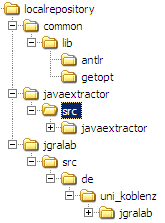
\includegraphics[width=4cm]{figures/repostructure-simplified.png}
	  \caption{Estimated directory structure for extractor usage (reduced to the relevant sub-structures).}
	  \label{repostructure}
  \end{center}
\end{figure}

\subsection{Classpath}
The usage of the extractor requires the following files and folders to be included in the \texttt{CLASSPATH}:
\begin{itemize}
	\item{The current directory (the extractors source code directory):\\
	\texttt{"."}}
	\item{The directory containing the source code of JGraLab:\\
	\texttt{"../../jgralab/src"}}
	\item{The GetOPT library used by some components of JGraLab:\\
	\texttt{"../../common/lib/getopt/java-getopt-1.0.13.jar"}}
	\item{The ANTLR library used by both JGraLab and the extractor itself:\\
	\texttt{"../../common/lib/antlr/org.antlr\_2.7.6.jar"}}
\end{itemize}
This can be achieved most easily by setting the according environment variable. The alternative way of passing the classpath over with the Java command line argument \texttt{-cp} is also possible, but for better readability this is not explored further in this document.

\subsection{Main call and parameters}
The main call of the extractor is done by executing:
\begin{lstlisting}
java javaextractor.JavaExtractor
\end{lstlisting}

In addition, the program accepts the following command line arguments (separated by spaces):
\begin{itemize}
	\item{\texttt{PATH} : The path of a file or a directory to be parsed. This argument may exist multiple times, but there must be at least one.}
	\item{\texttt{-out FILENAME} or \texttt{-o FILENAME} : The path of the file to which the generated graph will be written. \emph{.tg} is normally used as file name extension in GUPRO. This argument is optional, otherwise the graph is written to the file \emph{extractedgraph.tg} within the current directory by default. Existing files will be overwritten without warning.}
	\item{\texttt{-name PROGRAMNAME} or \texttt{-n PROGRAMNAME} : The name which is set as program name in the generated graph. This argument is optional.}
	\item{\texttt{-log FILENAME} oder \texttt{-l FILENAME} : The path of the file to which the log is written. This argument is optional, otherwise the file \emph{javaextractor.log} within the current directory will be used. An existing logfile will not be continued, but overwritten without warning.}
	\item{\texttt{-eager} or \texttt{-e} : Sets the extractor to eager mode, which means that it will try to build all informations in the graph which are required directly for references not included in the source code (by using reflection). This argument is optional.}
	\item{\texttt{-complete} or \texttt{-c} : Sets the extractor to eager mode, which means that it will try to build as many informations as possible in the graph for references not included in the source code (by using reflection). This argument is optional.}
\end{itemize}

\subsection{Increasing heap size}
It should be noted that a heap overflow is very likely to occur when processing a larger amount of source code with Java's default heap size. This may be avoided by increasing the maximum heap size using the command line argument \texttt{-Xmx}. Note that this is a command line argument of Java, not the extractor itself, which means that this argument must be the first one.

\subsection{Example call}
A call of the extractor with a maximum heap size of 768MB, using all the command line parameters mentioned above, might look as follows:
\begin{lstlisting}
java -Xmx768M javaextractor.JavaExtractor -out testgraph.tg -name Testprogramm -log testextract.log -eager ../testit/test1.java ../testit/test2.java ../testit2
\end{lstlisting}

\end{document}